\documentclass[xcolor=dvipsnames, notes=hide]{beamer}
%\documentclass[xcolor=dvipsnames, notes=only]{beamer}
%\documentclass[xcolor=dvipsnames]{beamer}
%\setbeameroption{show only notes}
%\usepackage{pgfpages}
%\setbeamertemplate{note page}[plain]
%\setbeameroption{show notes on second screen=right}

\usepackage[english]{babel}
\usepackage[utf8]{inputenc}
\usepackage[T1]{fontenc} % Ligaturen, richtige Umlaute im PDF

\newcommand{\backupbegin}{
	\newcounter{finalframe}
	\setcounter{finalframe}{\value{framenumber}}
}
\newcommand{\backupend}{
	\setcounter{framenumber}{\value{finalframe}}
}

\usepackage[absolute,overlay]{textpos} % textblock for figure placement

\usepackage{tabularx, booktabs}
\usepackage{amsmath}
\usepackage{blkarray, bigstrut}
\usepackage{xparse}

\usepackage[normalem]{ulem} % for \sout{}
\usepackage[ruled]{algorithm}
\usepackage{algpseudocode} 
\makeatletter
\def\BState{\State\hskip-\ALG@thistlm}
\algdef{SE}[DOWHILE]{Do}{doWhile}{\algorithmicdo}[1]{\algorithmicwhile\ #1}
\makeatother

\beamertemplatenavigationsymbolsempty
%\selectlanguage{english}
%\usepackage{biblatex}
%\bibliography{Bibliography}

\usepackage{bbm} % For mathbb{1}
\usepackage{csquotes}
\usepackage{colordvi}
\usepackage{xcolor}
%\usepackage{foiltex}

%\usepackage{enumitem}

\usepackage{tikz}
\usetikzlibrary{positioning}
\graphicspath{{/images/}}


\usetheme{CambridgeUS}
% Other valid themes
%   Antibes, Bergen, Berkeley, Berlin, Copenhagen
%   Darmstadt, Dresden, Frankfurt, Goettingen, Hannover
%   Ilmenau, JuanLesPins, Luebeck, Madrid, Malmoe
%   Marburg, Montpellier, PaloAlto, Pittsburgh, Rochester
%   Singapore, Szeged, Warsaw, boxes, default

%\usecolortheme{beetle}
%\usecolortheme{dolphin}
% Other valid color schemes
%    albatross, beaver, beetle, crane, dolphin
%    dove, fly, lily, orchid, rose, seagull
%    seahorse, whale and the one and only wolverine

%%%%%%%%%%%%%%%%%%%%%%%%%%%%%%%%
%%%%% PyCharm Color Scheme %%%%%
%%%%%%%%%%%%%%%%%%%%%%%%%%%%%%%%

%%% COLOR DEFINITIONS
\definecolor{uniBonnBlueDark}{HTML}{004F9F}
\definecolor{uniBonnYellow}{HTML}{F4B400} % lighter shades: FFDE85, FFD35C

\definecolor{pyCharmBgMain}{HTML}{2B2B2B} % RGB: 43, 43, 43

\definecolor{titleCardBg}{HTML}{CFCFEF} % former: F6511D (orange), CFCFEF (light purple) 

\definecolor{pyCharmBgSecond}{HTML}{313335}
\definecolor{pyCharmFgSecond}{HTML}{9F9FAF} % RGB: 159, 159, 175

\definecolor{pyCharmGreen}{HTML}{499C54} % RGB: 73, 156, 84
\definecolor{bfseriescolor}{HTML}{499C54}

%%% Original PyCharmColors:
%\definecolor{pyCharmBgMain}{HTML}{2B2B2B}
%\definecolor{pyCharmFgMain}{HTML}{88B1AC}
%\definecolor{pyCharmBgSecond}{HTML}{313335}
%\definecolor{pyCharmFgSecond}{HTML}{5D5F53}
%\definecolor{pyCharmGreen}{HTML}{499C54}

%%% COLOR SETTINGS
%\setbeamercolor{background canvas}{fg=pyCharmFgSecond, bg=pyCharmBgMain}
%\setbeamercolor{background}{fg=pyCharmFgSecond, bg=pyCharmBgMain}
%
%\setbeamercolor{normal text}{fg=pyCharmFgSecond,bg=pyCharmFgSecond}
%\setbeamercolor{alerted text}{fg=red}
%
\setbeamercolor{palette primary}{fg=pyCharmBgSecond, bg=white}
\setbeamercolor{palette secondary}{fg=pyCharmBgSecond, bg=white}
\setbeamercolor{palette tertiary}{fg=uniBonnBlueDark, bg=white}
%
\setbeamercolor{frametitle}{bg=titleCardBg, fg=uniBonnBlueDark} % Frametitle on every slide
\setbeamercolor{title}{fg=black, bg=titleCardBg}	% Title card slide
%
%\setbeamercolor{local structure}{fg=pyCharmGreen} % light green
%\setbeamercolor{subsection in toc}{bg=pyCharmBgMain, fg=pyCharmGreen}
%\setbeamercolor{section in toc}{bg=pyCharmBgMain, fg=pyCharmGreen}
%
%% For figure captions
%\setbeamercolor{caption}{fg=pyCharmFgSecond}
\setbeamercolor{caption name}{fg=pyCharmGreen}
%
%\setbeamertemplate{itemize item}{fg=pyCharmGreen$\blacksquare$}
%\setbeamertemplate{itemize subitem}{\color{499C54}$\blacksquare$}
%\setbeamertemplate{itemize items}[default]
%\setbeamertemplate{enumerate items}[default]

\setbeamertemplate{section in toc}{%
	{\color{pyCharmGreen} \inserttocsectionnumber.}\color{pyCharmFgSecond}~\inserttocsection}
\setbeamertemplate{subsection in toc}{%
	\hspace{1.2em}{\color{pyCharmGreen}\rule[0.3ex]{3pt}{3pt}} ~\inserttocsubsection\par}

\renewcommand{\textbf}[1]{{\bfseries\color{bfseriescolor}#1}}
%
\setbeamercolor*{palette tertiary}{bg=uniBonnBlueDark}

%%% Numbersets
\newcommand{\eye}{\mathbb{1}} % Identitiy matrix
\newcommand{\one}{\textbf{1}} % One-vector (1 1 ... 1)
\newcommand{\IN}{\mathbb{N}} % Natural numbers
\newcommand{\IR}{\mathbb{R}} % Real numbers
\newcommand{\IZ}{\mathbb{Z}} % Integers
\newcommand{\IQ}{\mathbb{Q}} % Rational numbers
\newcommand{\ID}{\mathbb{D}} % Dyadic numbers
\newcommand{\IC}{\mathbb{C}} % Complex numbers
\newcommand{\IF}{\mathbb{F}} % (Vector) Field
%\newcommand{\vA}{\mathcal{A}}
%\newcommand{\vD}{\mathcal{D}}
%\newcommand{\vB}{\mathcal{B}}
%\newcommand{\vP}{\mathcal{P}}
%\newcommand{\vJ}{\mathcal{J}}
%\newcommand{\vU}{\mathcal{U}}
%%% Basic operators
\newcommand{\IP}{\mathbb{P}} % Probability operator
\newcommand{\IE}{\mathbb{E}} % Expectation operator
\newcommand{\vF}{\mathcal{F}} % Fourier transform
%%% Distributions
\newcommand{\vN}{\mathcal{N}} % Normal distribution
\newcommand{\Bin}{\mathop{\mathrm{Bin}}} % Binomial distribution
\newcommand{\Poi}{\mathop{\mathrm{Poi}}} % Poisson distribution
%%% Others
\newcommand{\Cov}{\mathop{\mathrm{Cov}}} % covariance
\newcommand{\co}{\mathop{\mathrm{co}}} % covariance
\newcommand{\Var}{\mathop{\mathrm{Var}}} % variance
\newcommand{\norm}[1]{\left\lVert#1\right\rVert} % norm
\newcommand{\var}[1]{{\ttfamily#1}} % variable
\newcommand{\tr}{\mathop{\operatorname{tr}}} % trace
\newcommand{\rk}{\mathop{\operatorname{rk}}} % rank
\newcommand{\diag}{\mathop{\operatorname{diag}}} % diagonal
\renewcommand{\vec}[1]{\bm{#1}} % vector
\newcommand{\mat}[1]{\bm{#1}} % matrix
\newcommand{\ten}[1]{\bm{\mathcal{#1}}}
\newcommand{\inv}[1]{#1^{-1}} % inverse
\newcommand{\trn}[1]{#1^\intercal} % transpose
\newcommand{\opt}[2]{#1 \trn{#2}} % outer product
\newcommand{\ipt}[2]{\trn{#1} #2} % inner product
\newcommand{\angles}[2]{\langle #1, #2 \rangle} % scalar product
\newcommand{\Angles}[2]{\bigl \langle #1, #2 \bigr \rangle} % big scalar product
\newcommand{\st}{\operatorname{s.\!t.}} % 'such that'
%%% Stacked symbols
\newcommand{\amin}[1]{\operatorname*{argmin}_{#1}}
\newcommand{\amax}[1]{\operatorname*{argmax}_{#1}}
\newcommand{\sign}{\mathop{\mathrm{sign}}}
\newcommand{\eqex}{\mathop{\stackrel{!}{=}}}
\newcommand{\geex}{\mathop{\stackrel{!}{\ge}}}
\newcommand{\leex}{\mathop{\stackrel{!}{\le}}}
\newcommand{\softmax}{\operatorname*{softmax}}
%%% Table colors
\newcommand\cellr{\cellcolor{red!20}}
\newcommand\cellg{\cellcolor{green!10}}
\newcommand\cellb{\cellcolor{blue!10}}
\newcommand\cello{\cellcolor{orange!10}}
%%% Sets
\newcommand{\set}[1]{\{{#1}\}}
\newcommand{\Set}[1]{\big\{{#1}\big\}}
\newcommand{\BigSet}[1]{\Big\{{#1}\Big\}}
%%% Multisets
\newcommand{\mset}[1]{\{\mskip-5mu\{{#1}\}\mskip-5mu\}}
\newcommand{\Mset}[1]{\big\{\mskip-5mu\big\{{#1}\big\}\mskip-5mu\big\}}
\newcommand{\BigMset}[1]{\Big\{\mskip-5mu\Big\{{#1}\Big\}\mskip-5mu\Big\}}
%%% Footnote
%\deffootnote{1.5em}{1em}{\makebox[1.5em][l]{\thefootnotemark}}

%%% LOGO PLACEMENT
\addtobeamertemplate{frametitle}{}{%
	\begin{tikzpicture}[remember picture,overlay]
	\node[anchor=north east,yshift=-3pt] at (current page.north east) {
		
\includegraphics[height=0.8cm]{images/UNI_Bonn_Logo_Standard_RZ_XL.png}
		
\includegraphics[height=0.8cm]{images/AG_logo_hp_70x70.png}
	};
	\end{tikzpicture}}
%\addtobeamertemplate{frametitle}{}{%
%	\begin{tikzpicture}[remember picture,overlay]
%	\node[anchor=north east,yshift=-9pt] at (current page.north east) {
%		
\includegraphics[height=0.8cm]{images/UNI_Bonn_Logo_Standard_RZ_XL.png}
%		
\includegraphics[height=0.8cm]{images/AG_logo_hp_70x70.png}
%	};
%	\end{tikzpicture}}
% !Tex spellceck = en_US

\title[MA Seminar Talk - Progress]{
	\centering
	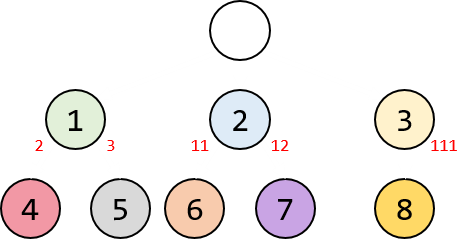
\includegraphics[width=0.3\textwidth]{images/WLLT}\\
	Master Thesis Seminar Talk	
}
%\title[MA Seminar Talk - Progress]{Master Thesis Seminar Talk}
%\titlegraphic{
%	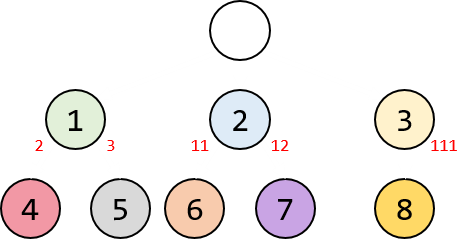
\includegraphics[width=0.2\textwidth]{images/WLLT}
%}
\subtitle{Progress Update}
\author[F. Beaumont]{Fabrice Beaumont}
\institute[]{Department of Information Systems and Artificial Intelligence - \textbf{Dr. Pascal Welke}}
\date{10. November 2022}

\newcommand{\figureWidth}{7cm}
\newcommand{\figureHorizontal}{2cm}
\newcommand{\figureVertical}{5cm}
%\setbeamersize{text margin left=0pt,text margin right=0pt}
\begin{document}

\begin{frame}
	\titlepage
\end{frame}

%%%%%%%%%%%%%%%%%%%%%%%%%%%%%%%%%%%%%%%%%%%%%%%%%%%%%%%%%%%%%%%%%%%%%%%%%
\section{Method}


\begin{frame}
\frametitle{Example of the whole procedure}
\centering
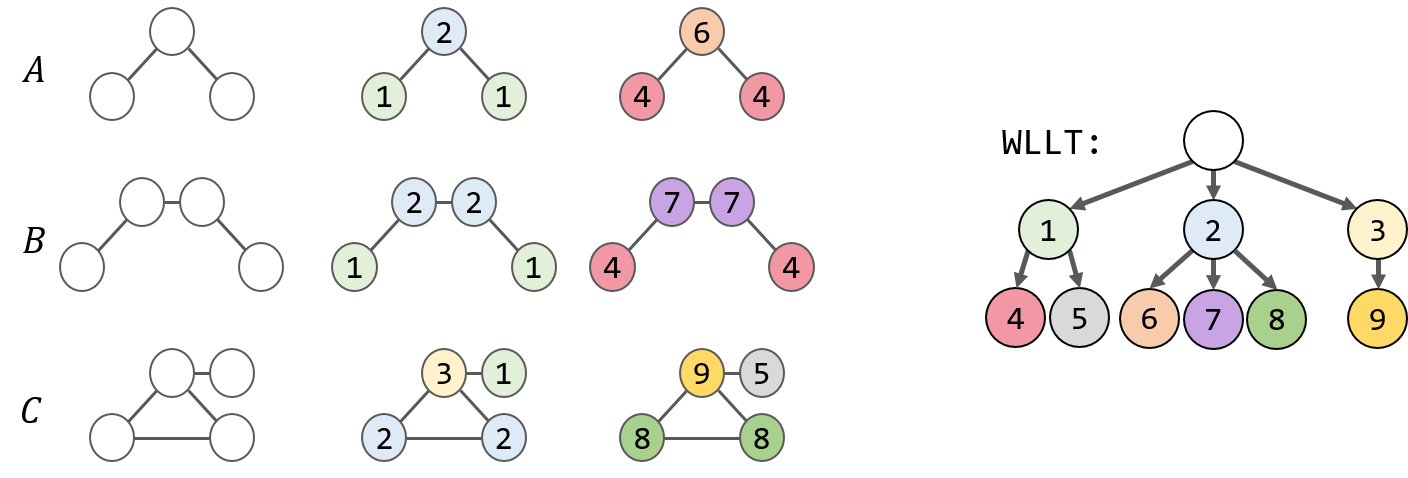
\includegraphics[width=0.8\textwidth]{images/WL_labeling_iterations}
\end{frame}


\begin{frame}
	\frametitle{Example of the whole procedure}\vspace{-0.75cm}
	\centering
	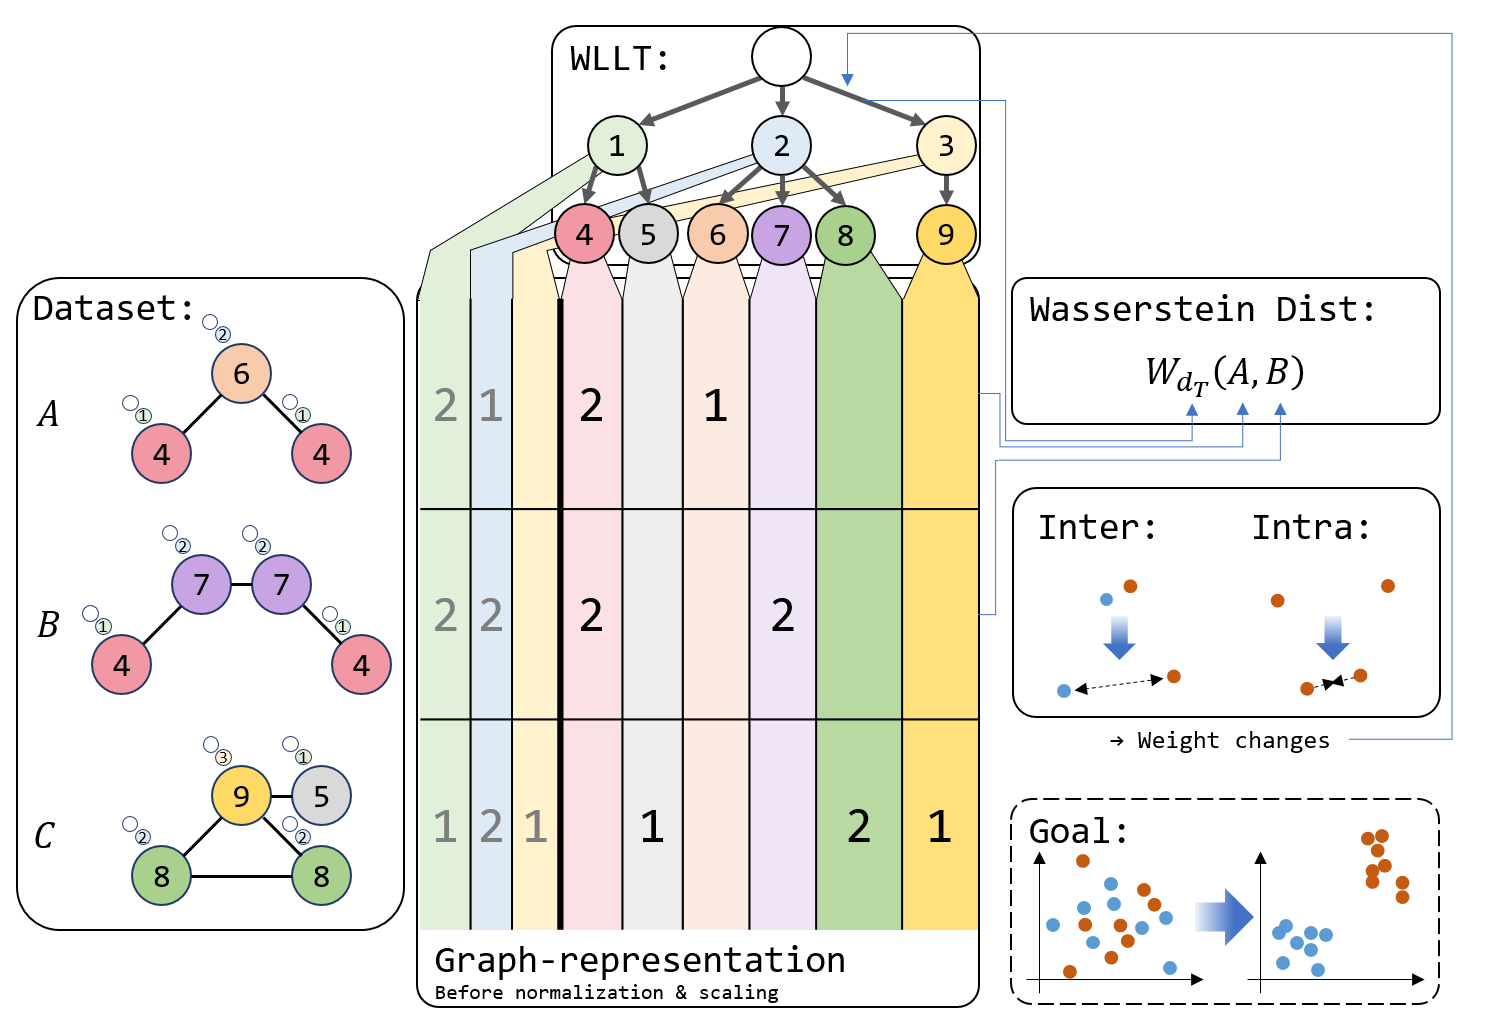
\includegraphics[width=0.9\textwidth]{images/WLLTProgram6}
\end{frame}

\section{Results}

\begin{frame}\frametitle{Example: AIDS t-SNE}
	\begin{minipage}{0.49\textwidth}
		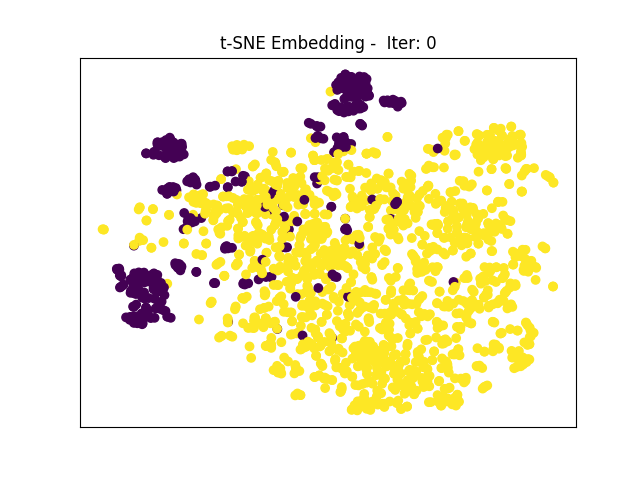
\includegraphics[width=\textwidth]{images/plot8tSNE}
	\end{minipage}
	\begin{minipage}{0.49\textwidth}
		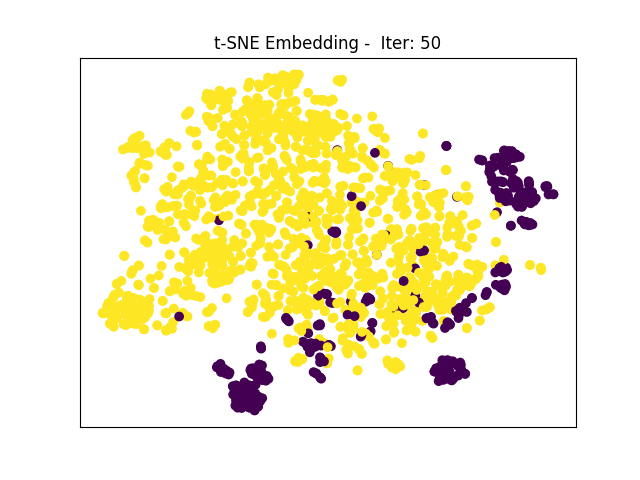
\includegraphics[width=\textwidth]{images/plot9tSNE}
	\end{minipage}
\vspace{2cm} \\
\tiny{Bs: $5\%$, WLLT-d: $4$, PP: $0.4$, SVM-acc.: $80\%$}
\end{frame}

\begin{frame}\frametitle{Example: NCI1 t-SNE}
	\begin{minipage}{0.49\textwidth}
		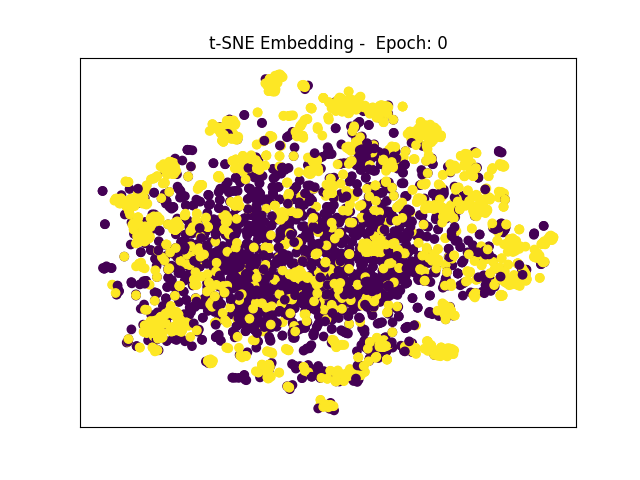
\includegraphics[width=\textwidth]{images/plot10tSNE}
	\end{minipage}
	\begin{minipage}{0.49\textwidth}
		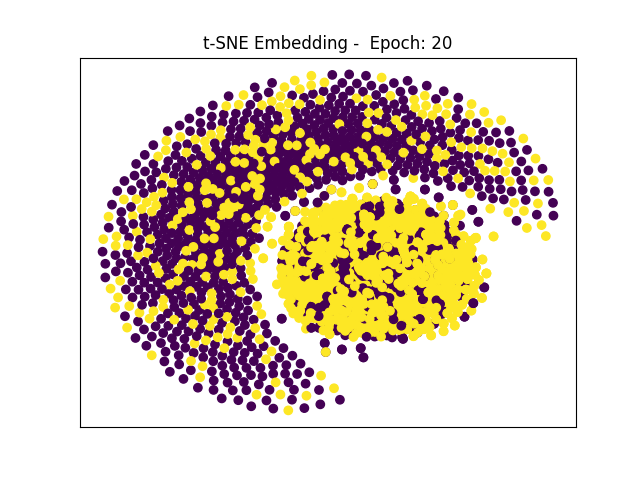
\includegraphics[width=\textwidth]{images/plot11tSNE}
	\end{minipage}
	\vspace{2cm} \\
	\tiny{Bs: $5\%$, WLLT-d: $4$, Pull: $1.0$, Push: $0.1$, SVM-acc.: $48\%$}
\end{frame}

\begin{frame}\frametitle{Example: NCI1 t-SNE}
	\begin{minipage}{0.49\textwidth}
		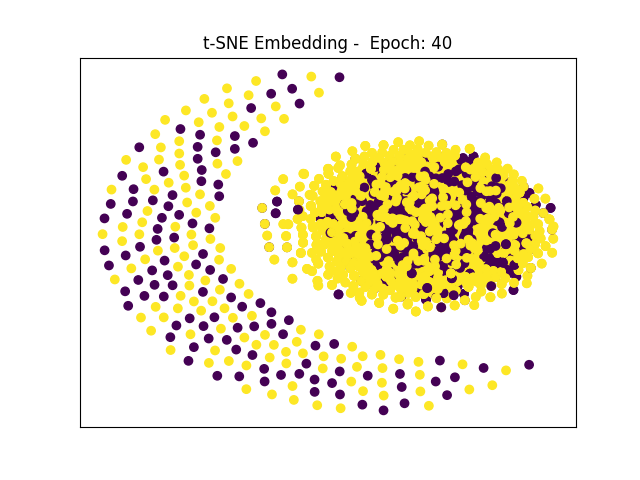
\includegraphics[width=\textwidth]{images/plot12tSNE}
	\end{minipage}
	\begin{minipage}{0.49\textwidth}
		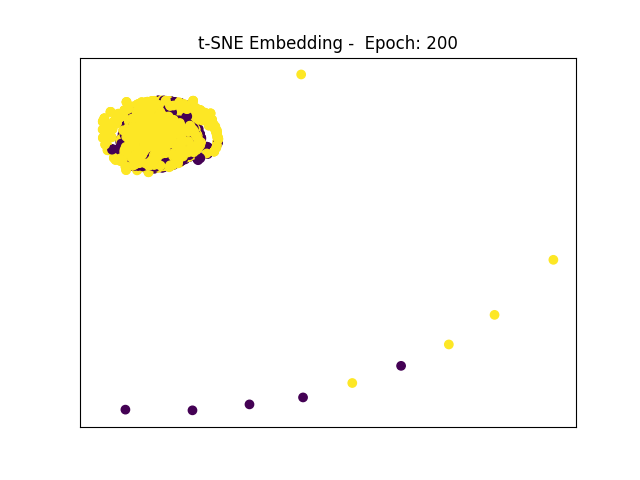
\includegraphics[width=\textwidth]{images/plot13tSNE}
	\end{minipage}
	\vspace{2cm} \\
	\tiny{Bs: $5\%$, WLLT-d: $4$, Pull: $1.0$, Push: $0.1$, SVM-acc.: $48\%$}
\end{frame}

\begin{frame}\frametitle{Example: ENZYMES t-SNE}
	\begin{minipage}{0.49\textwidth}
		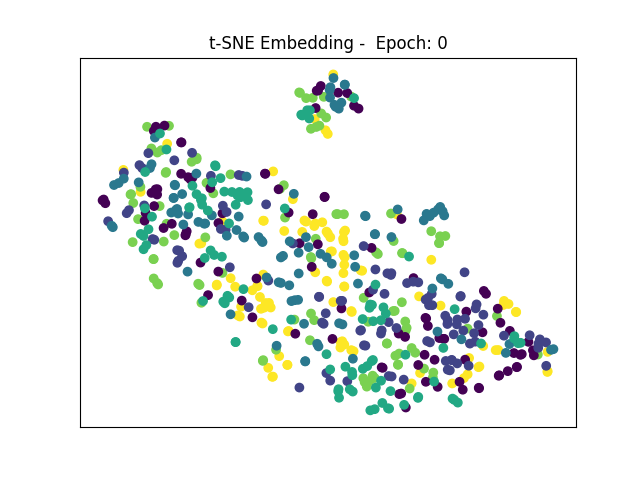
\includegraphics[width=\textwidth]{images/plot14tSNE}
	\end{minipage}
	\begin{minipage}{0.49\textwidth}
		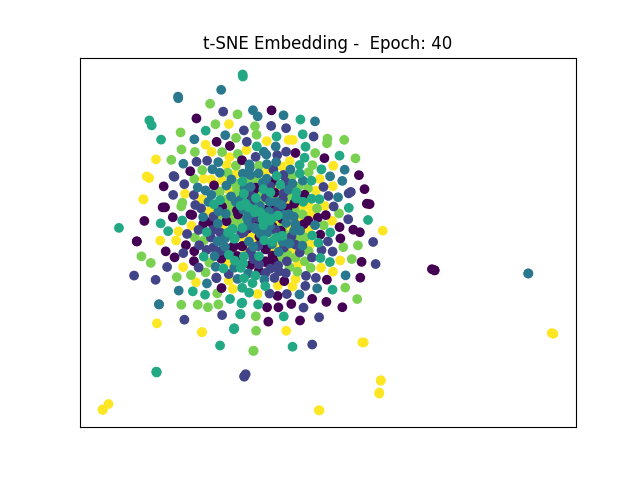
\includegraphics[width=\textwidth]{images/plot15tSNE}
	\end{minipage}
	\vspace{2cm} \\
	\tiny{Bs: $5\%$, WLLT-d: $4$, Pull: $1.0$, Push: $0.1$, SVM-acc.: $11\%$}
\end{frame}

\begin{frame}\frametitle{Example: ENZYMES t-SNE}
	\begin{minipage}{0.49\textwidth}
		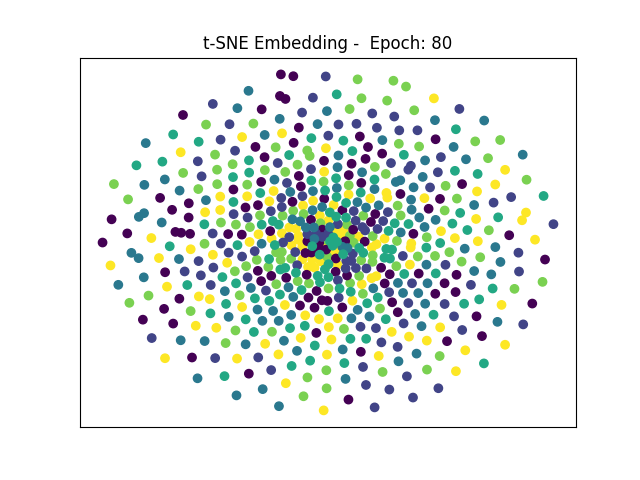
\includegraphics[width=\textwidth]{images/plot16tSNE}
	\end{minipage}
	\begin{minipage}{0.49\textwidth}
		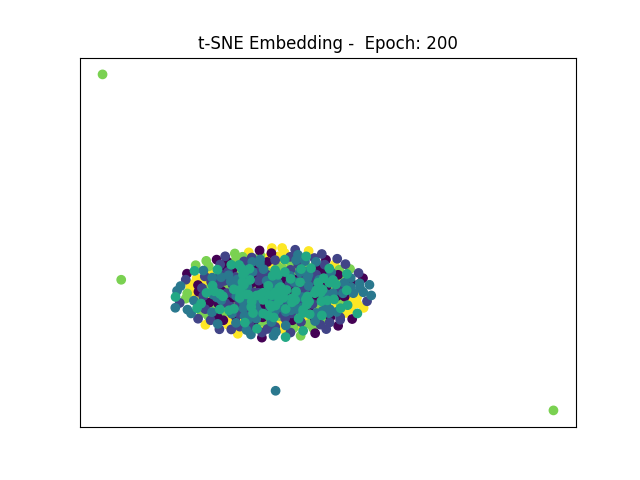
\includegraphics[width=\textwidth]{images/plot17tSNE}
	\end{minipage}
	\vspace{2cm} \\
	\tiny{Bs: $5\%$, WLLT-d: $4$, Pull: $1.0$, Push: $0.1$, SVM-acc.: $11\%$}
\end{frame}

\begin{frame}\frametitle{Example: Sample movement error}
	\begin{minipage}{0.49\textwidth}
		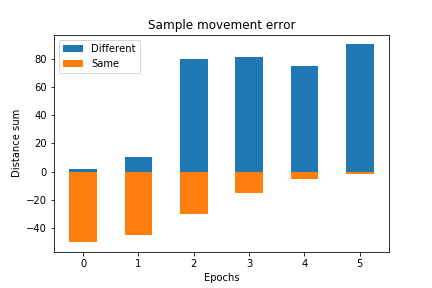
\includegraphics[width=\textwidth]{images/IdealSME}
	\end{minipage}
	\begin{minipage}{0.49\textwidth}
		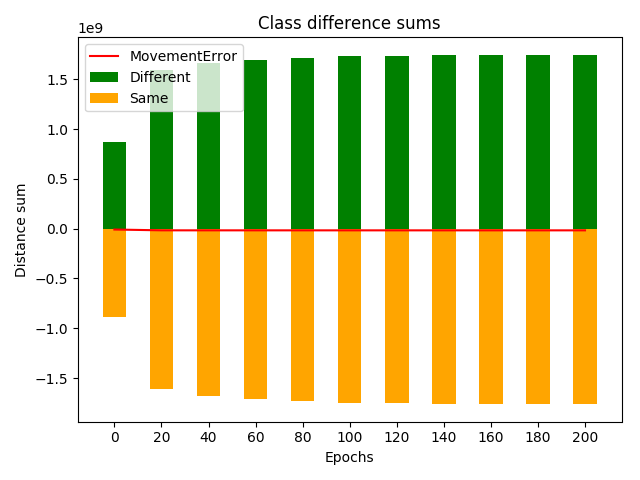
\includegraphics[width=\textwidth]{images/plot18ClDiffSums}
	\end{minipage}
	\vspace{2cm} \\
	\tiny{NCI1, Bs: $5\%$, WLLT-d: $4$, Pull: $0.1$, Push: $0.5$, SVM-acc.: $48\%$}
\end{frame}

\begin{frame}\frametitle{Example: Sample movement error}
	\begin{minipage}{0.49\textwidth}
		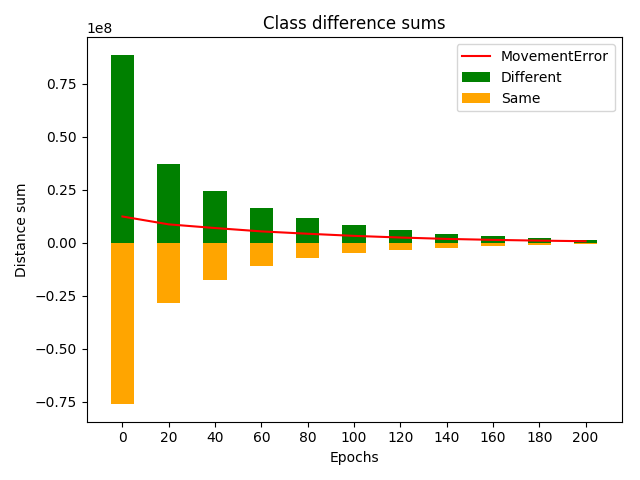
\includegraphics[width=\textwidth]{images/plot19ClDiffSums}
	\end{minipage}
	\begin{minipage}{0.49\textwidth}
		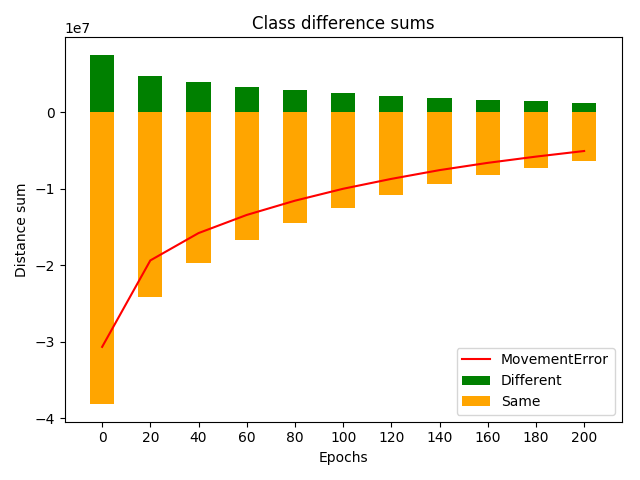
\includegraphics[width=\textwidth]{images/plot20ClDiffSums}
	\end{minipage}
	\vspace{2cm} \\
	\tiny{PROTEINS\_c, Bs: $5\%$, WLLT-d: $4$, Pull: $1.0$, Push: $0.1$, SVM-acc.: $64\%$}\\
	\tiny{ENZYMES, Bs: $5\%$, WLLT-d: $4$, Pull: $1.0$, Push: $0.1$, SVM-acc.: $11\%$}
\end{frame}


\begin{frame}\frametitle{Example: Sample movement error}
	\begin{minipage}{0.4\textwidth}
		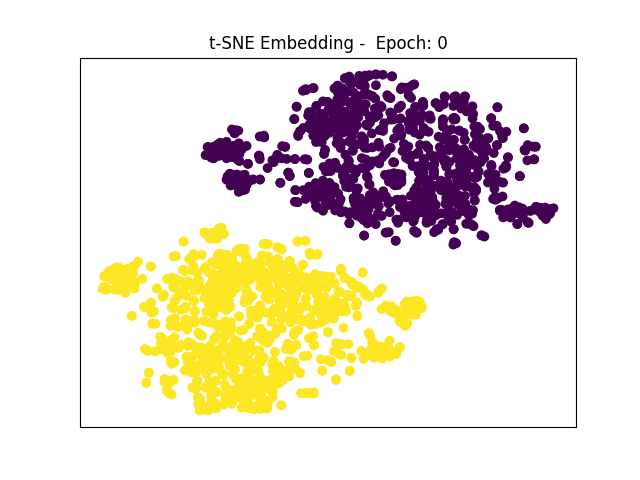
\includegraphics[width=\textwidth]{images/plot21tSNE}
	\end{minipage}
	\begin{minipage}{0.4\textwidth}
		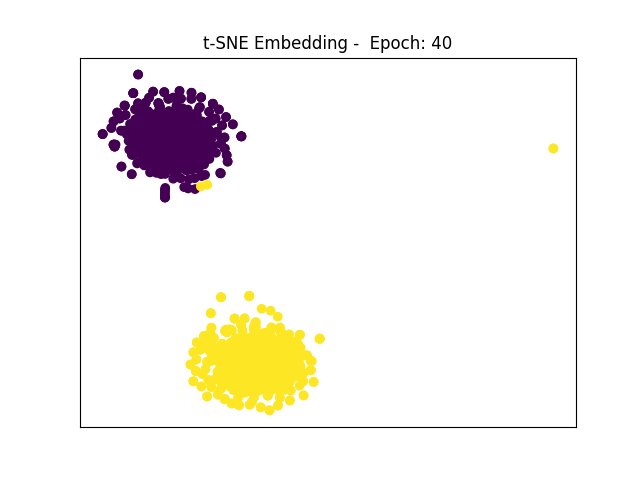
\includegraphics[width=\textwidth]{images/plot22tSNE}
	\end{minipage}

	\begin{minipage}{0.4\textwidth}
		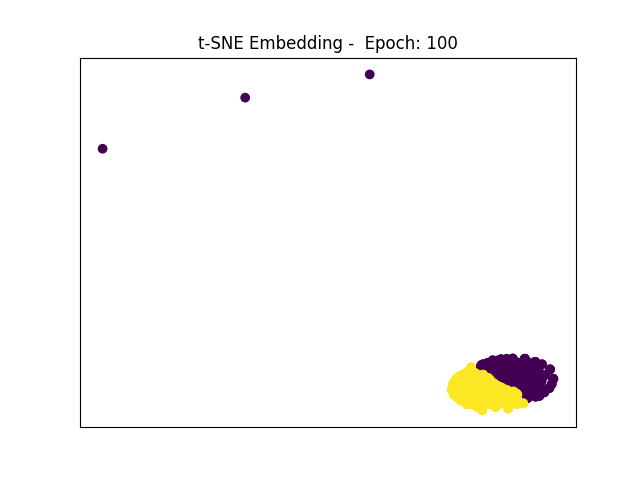
\includegraphics[width=\textwidth]{images/plot23tSNE}
	\end{minipage}
	\begin{minipage}{0.4\textwidth}
		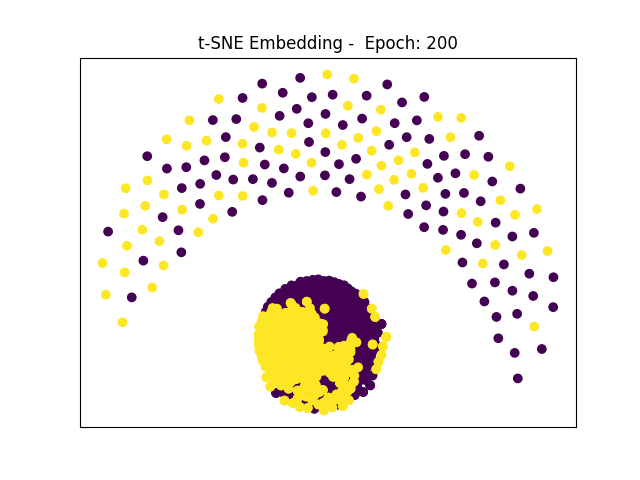
\includegraphics[width=\textwidth]{images/plot24tSNE}
	\end{minipage}
	\vspace{2cm} \\
	\tiny{AIDS\_perfect, Bs: $5\%$, WLLT-d: $4$, Pull: $0.3$, Push: $0.1$, SVM-acc.: $51\%$}
\end{frame}

\begin{frame}\frametitle{Example: AIDS\_perfect}
	Separate clusters for:\\
	\begin{center}
		WLLT-d=$4$, $100$ epochs, Bs=$5\%$, He\_thdl=$0.6$, Pull=$0.1$, Push=$0.1$
	\end{center}
	And with changed:
	\begin{itemize}
		\item Bs=$20\%$
		\item WLLT-d=$2$
		\item Lr=$0.5$
	\end{itemize}	
	Assume that these parameters do not interfere with the cluster separation.\\
	Suspect instead the scaling effect of multiplicative updates. Thus try absolute updates.
\end{frame}


\begin{frame}\frametitle{Example: AIDS\_perfect - SVM accuracy}
	Expected (almost) $100\%$ for iteration 0. But got only \textcolor{red}{$51\%$}.\newline
	
	Testing the SVM with other \textbf{kernel lambdas} $\lambda$ besides the standard 'scale' in the computation of the kernel matrix from the distance matrix $D$:
	\[ K := \exp(-\lambda D) \]
	\begin{center}\begin{tabular}{l|r r r r r}
		$\lambda$ & scale 	& \textbf{auto} & $0.1$ & $0.5$ & $1.0$\\ \hline
		Avg.Acc.  & $50.43$ & 97.94 & 79.99 & 50.54 &  50.91\\
		Std.dev.  &  $3.69$ &  2.53 &  1.26 &  0.93 &  0.55
	\end{tabular}\end{center}
	Where:
	\begin{itemize}
		\item auto:  $\lambda = 1 / \big(\#\{\text{features}\} * \operatorname{var}(D)\big)$
		\item scale: $\lambda = 1 / (\#\{\text{features}\})$ 
	\end{itemize}
	'scale' is the default of sklearn's svm implementation (since version $0.22$).
\end{frame}

%%%%%%%%%%%%%%%%%%%%%%%%%%%%%%%%%%%%%%%%%%%%%%%%%%%%%%%%%%%%%%%%%%%%%%%%%
\section{Outlook}

\begin{frame}\frametitle{Outlook}
	\begin{itemize}
		\item \enquote{Finish} experiments with \texttt{AIDS\_perfect}\\
		(limits of push-pull, absolute weight update, single layer)
		\item Try to find more truly SME improving configuration for (normal) AIDS\\
		(Ideally increasing diff-cl distance \textbf{and} decreasing same-cl dist.)
		\item[]
		\item Besides this: \textbf{Terminate the evaluations} and report about the investigated parameter configurations.\\
		Outlook for improvement of the method: e.g. Layer gradient
	\end{itemize}	
\end{frame}

\section{Outlook - Usage}
\begin{frame}\frametitle{Example: MUTAG WLLT layer 0}
	\begin{minipage}{0.49\textwidth}
		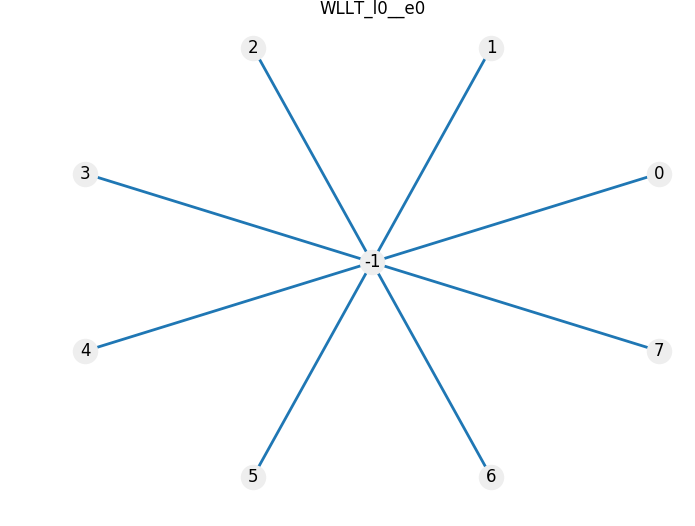
\includegraphics[width=\textwidth]{images/plotWlltl0}
	\end{minipage}
	\begin{minipage}{0.49\textwidth}
		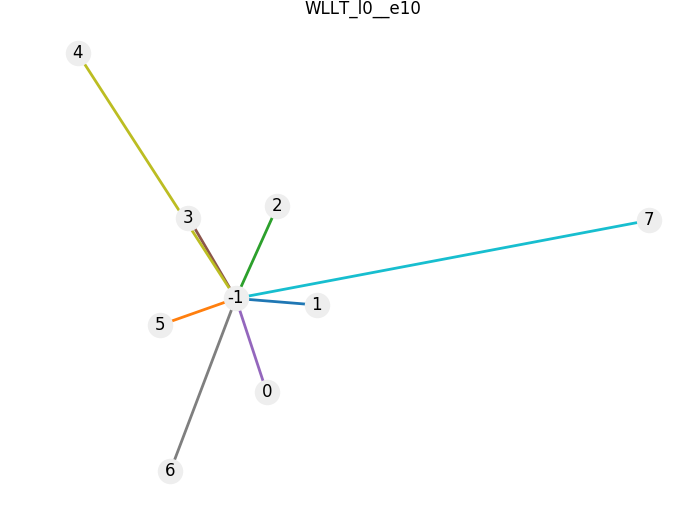
\includegraphics[width=\textwidth]{images/plotWlltl1}
	\end{minipage}
	\vspace{2cm} \\
	\tiny{Bs: $20\%$, WLLT-d: $4$, Pull: $0.3$, Push: $0.1$, SVM-acc.: $66\%$}
\end{frame}

\begin{frame}\frametitle{Example: MUTAG WLLT layer 1}
	\begin{minipage}{0.49\textwidth}
		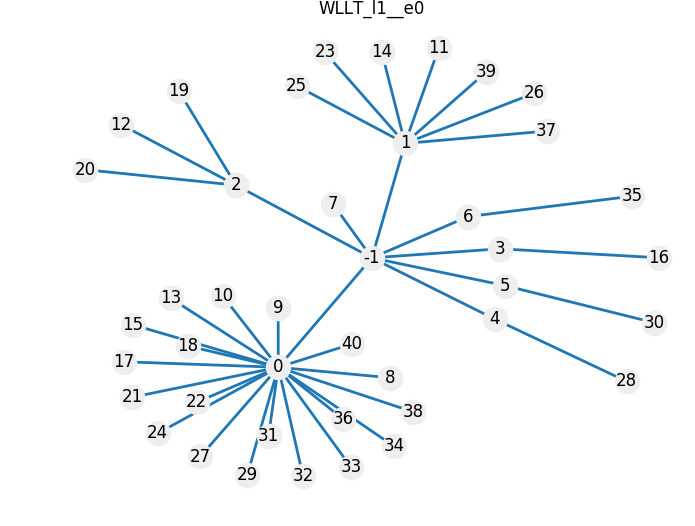
\includegraphics[width=\textwidth]{images/plotWlltl2}
	\end{minipage}
	\begin{minipage}{0.49\textwidth}
		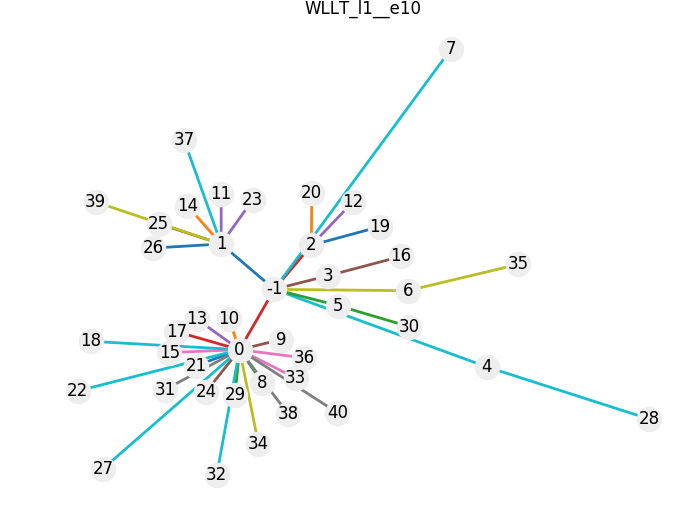
\includegraphics[width=\textwidth]{images/plotWlltl3}
	\end{minipage}
	\vspace{2cm} \\
	\tiny{Bs: $20\%$, WLLT-d: $4$, Pull: $0.3$, Push: $0.1$, SVM-acc.: $66\%$}
\end{frame}

\begin{frame}\frametitle{Example: MUTAG WLLT layer 2}
	\begin{minipage}{0.49\textwidth}
		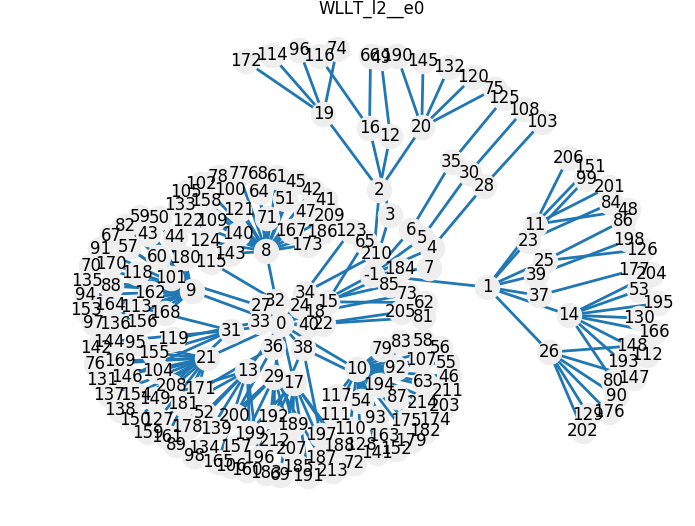
\includegraphics[width=\textwidth]{images/plotWlltl4}
	\end{minipage}
	\begin{minipage}{0.49\textwidth}
		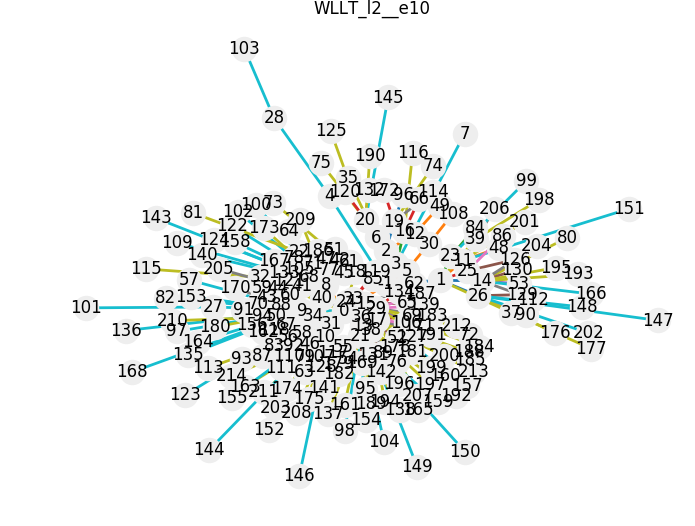
\includegraphics[width=\textwidth]{images/plotWlltl5}
	\end{minipage}
	\vspace{2cm} \\
	\tiny{Bs: $20\%$, WLLT-d: $4$, Pull: $0.3$, Push: $0.1$, SVM-acc.: $66\%$}
\end{frame}

\begin{frame}\frametitle{Example: AIDS WLLT layer 2}
	\begin{minipage}{0.49\textwidth}
		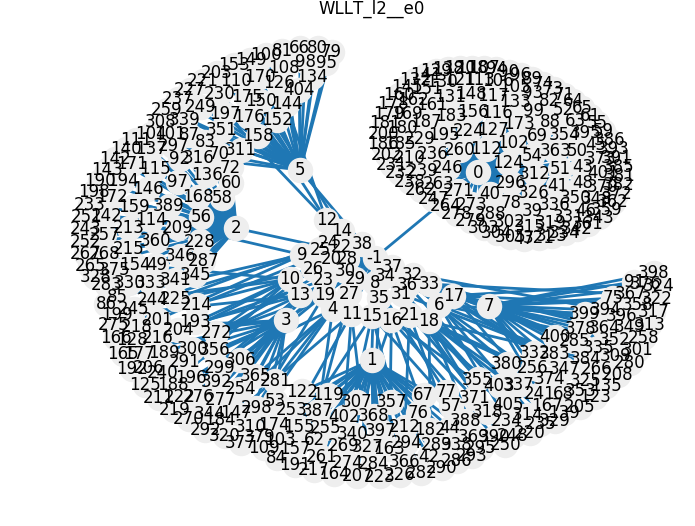
\includegraphics[width=\textwidth]{images/plot6wllt}
	\end{minipage}
	\begin{minipage}{0.49\textwidth}
		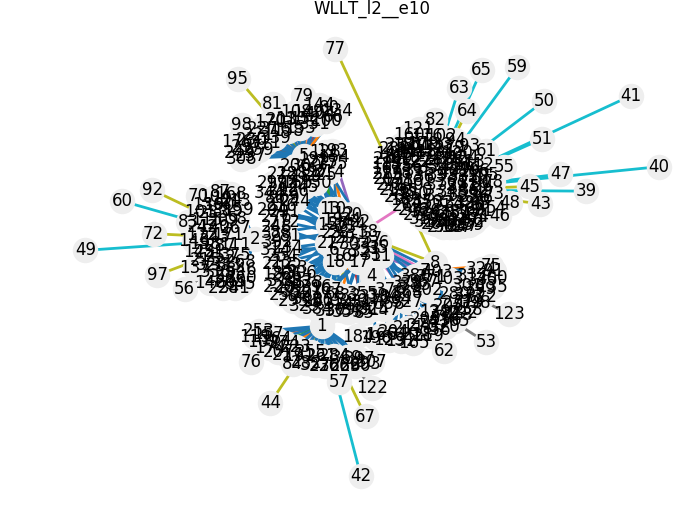
\includegraphics[width=\textwidth]{images/plot7wllt}
	\end{minipage}
	\vspace{2cm} \\
	\tiny{Bs: $5\%$, WLLT-d: $4$, PP: $0.4$, SVM-acc.: $80\%$}
\end{frame}

%%%%%%%%%%%%%%%%%%%%%%%%%%%%%%%%%%%%%%%%%%%%%%%%%%%%%%%%%%%%%%%%%%%%%%%%%
\section{End}

\begin{frame}[c]
	\centering %\Huge
	\begin{huge}
		\emph{Thank you all for listening.}\\
	\end{huge}
	\vspace{2 cm}
	I will be happy to answer any \textbf{questions} and\\
	hear your \textbf{comments}.
\end{frame}

%%%%%%%%%%%%%%%%%%%%%%%%%%%%%%%%%%%%%%%%%%%%%%%%%%%%%%%%%%%%%%%%%%%%%%%%%
\appendix
\section{Appendix}

\begin{frame}[noframenumbering]
	\frametitle{Preparation of the performance comparison}	
	\begin{figure}
		\centering
		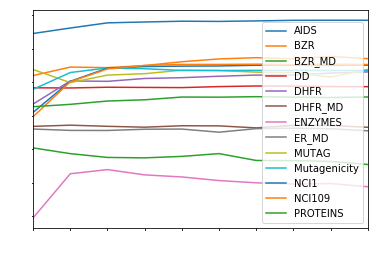
\includegraphics[width=0.6\linewidth]{images/plot_whiteText}
		\caption{Classification accuracies on databases using Weisfeiler-Lehman.}
		\label{fig:plot}
	\end{figure}
	\tiny{\texttt{grakel.kernels.\textbf{WeisfeilerLehman}(n\_iter=[1-10], base=grakel.kernels.VertexHistogram, normalize=True)}}\\
	\tiny{\texttt{grakel.utils.\textbf{cross\_validate\_Kfold\_SVM}(K, y, n\_iter=10)}}

\end{frame}

\end{document}